% \iffalse
\let\negmedspace\undefined
\let\negthickspace\undefined
\documentclass[journal,12pt,twocolumn]{IEEEtran}
\usepackage{cite}
\usepackage{amsmath,amssymb,amsfonts,amsthm}
\usepackage{algorithmic}
\usepackage{graphicx}
\usepackage{textcomp}
\usepackage{xcolor}
\usepackage{txfonts}
\usepackage{listings}
\usepackage{enumitem}
\usepackage{mathtools}
\usepackage{gensymb}
\usepackage{comment}
\usepackage[breaklinks=true]{hyperref}
\usepackage{tkz-euclide} 
\usepackage{listings}
\usepackage{gvv}                                        
\def\inputGnumericTable{}                                 
\usepackage[latin1]{inputenc}                                
\usepackage{color}                                            
\usepackage{array}                                            
\usepackage{longtable}                                       
\usepackage{calc}                                             
\usepackage{multirow}                                         
\usepackage{hhline}                                           
\usepackage{ifthen}                                           
\usepackage{lscape}
\usepackage{placeins}
\usepackage{xparse}


\newtheorem{theorem}{Theorem}[section]
\newtheorem{problem}{Problem}
\newtheorem{proposition}{Proposition}[section]
\newtheorem{lemma}{Lemma}[section]
\newtheorem{corollary}[theorem]{Corollary}
\newtheorem{example}{Example}[section]
\newtheorem{definition}[problem]{Definition}
\newcommand{\BEQA}{\begin{eqnarray}}
\newcommand{\EEQA}{\end{eqnarray}}
\newcommand{\define}{\stackrel{\triangle}{=}}
\theoremstyle{remark}
\newtheorem{rem}{Remark}

\graphicspath{ {./figs/} } 

\begin{document}

\bibliographystyle{IEEEtran}
\vspace{3cm}

\Large\title{NCERT Question 10.5.2.5}
\large\author{EE23BTECH11032 - Kaustubh Parag Khachane $^{*}$% <-this % stops a space
}
\maketitle
\newpage
\bigskip

\renewcommand{\thefigure}{\theenumi}
\renewcommand{\thetable}{\theenumi}
\large\textbf{Question 10.5.2.5} : \normalsize Find the number of terms in each of the following APs. Then express each term as x(n) and find the z transform, ROC and plot the graph for x\brak{n}: 
\begin{enumerate}
    \item 7, 13, 19, ... 205

    \item 18, 15$\frac{1}{2}$, 13, ... -47
\end{enumerate}



\large\textbf{Solution} :\normalsize

\begin{table}[!ht] 
\centering
\setlength{\extrarowheight}{8pt}
\begin{tabular}{|l|l|l|}
    \hline
    \textbf{Parameter} & \textbf{Description} & \textbf{Value} \\
    \hline
     m & Mass of object & 10 Kg \\\hline
     $\mu$ & Frictional coefficient \brak{static} & 0.25\\\hline
     x\brak{t} & Displacement of block &  \\\hline
     $x\brak{0}$ & Initial displacement & 0 \brak{assumed} \\\hline
     g & Gravitational acceleration & 10 $m/s^2$ \\\hline
     $F_s$ & Spring force &  \\\hline
     f & frictional force &  $\mu$ N \\\hline
     N & Normal Force & mg $cos\brak{\theta}$ \\\hline
    \end{tabular}
  \vspace{4mm}
 \caption{Parameter Table}
 \label{tab:table0_xe80}
\end{table}

The number of terms in the AP x(n) is given by: 
\begin{align}  \label{eq:eq12}
    \frac{x\brak{n} - x\brak{0}}{d} + 1
    \end{align}
\begin{align}
    &X_i(z) = \frac{x_i\brak{0}}{1 - z^{-1}} + d_i\frac{z^{-1}}{\brak{1-z^{-1}}^2} \text{ , for i=1,2} \label{eq:eq3}\\
    &\text{ROC : $\abs{z} > 1$ as it is an AP}   
\end{align}
\begin{enumerate}
    \item 
\begin{align}
x_{1}\brak{n} &= \brak{7 + \brak{n}6}u\brak{n}
\end{align}
Using the values in \tabref{table0} and equation \eqref{eq:eq12},
\begin{align}
    k_1 = \frac{205 - 7}{6} + 1 = 34
\end{align}

Using the values in \tabref{table0} and equation \eqref{eq:eq3} :
\begin{align}
 X_1\brak{z} = \frac{7 - z^{-1}}{\brak{1-z^{-1}}^2} , \abs{z} > 1
 \end{align}
 
\item
\begin{align}
x_{2}\brak{n} &= \brak{18 + n\brak{-2\frac{1}{2}}}u\brak{n}
 \end{align}
 Using the values in \tabref{table0} and equation \eqref{eq:eq12},
\begin{align}
    k_2 = \frac{-47 - 18}{-2.5} + 1 = 27
\end{align}
Using the values in \tabref{table0} and equation \eqref{eq:eq3} :
\begin{align} 
 X_2\brak{z} = \frac{18 - \brak{20.5}z^{-1}}{\brak{1 - z^{-1}}^2} , \abs{z} > 1
\end{align}


\begin{figure}[!ht]
\centering
\begin{center}
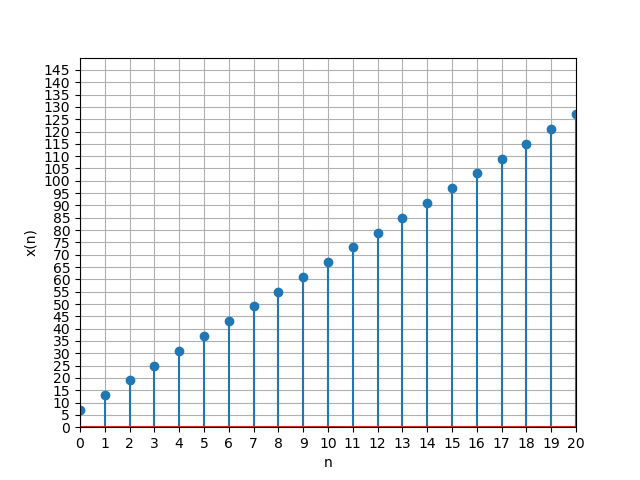
\includegraphics[width=\columnwidth]{Figure_1}
\caption{Plot of $x_1\brak{n}$}
\end{center}
\end{figure}

\begin{figure}[!ht]
\centering
\begin{center}
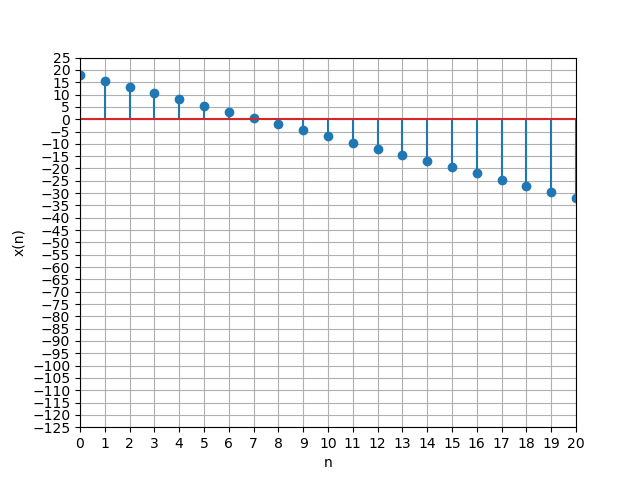
\includegraphics[width=\columnwidth]{Figure_2}
\caption{Plot of $x_2\brak{n}$}
\end{center}
\end{figure}

\end{enumerate}
\end{document}
